\documentclass{acm_proc_article-sp}
\usepackage{times}
\usepackage{url}
\usepackage{graphics}
\usepackage{color}
\newcommand{\want}[1]{}
\newcommand{\idea}[1]{}
\newcommand{\note}[1]{}
\newcommand{\x}[1]{}
\newcommand{\todo}[1]{}
\newcommand{\maybe}[1]{}
\newcommand{\resolved}[1]{}

% Mark up a point that we want to flesh out into more text
%\newcommand{\x}[1]{{\color{blue} #1}\\}

% Mark up some work that we need to do in order for this paper to be telling the truth
%\newcommand{\todo}[1]{{\color{red} #1}\\}

%\newcommand{\maybe}[1]{}

\begin{document}

\toappear

\bibliographystyle{plain}

\title{What is disputed on the web?}

%%
%% Note on formatting authors at different institutions, as shown below:
%% Change width arg (currently 7cm) to parbox commands as needed to
%% accommodate widest lines, taking care not to overflow the 17.8cm line width.
%% Add or delete parboxes for additional authors at different institutions. 
%% If additional authors won't fit in one row, you can add a "\\"  at the
%% end of a parbox's closing "}" to have the next parbox start a new row.
%% Be sure NOT to put any blank lines between parbox commands!
%%

\numberofauthors{5}

\author{
\alignauthor Rob Ennals\\
       \affaddr{Intel Labs Berkeley}\\
       \affaddr{2150 Shattuck Ave}\\
       \affaddr{Berkeley, CA, USA}\\
       \email{robert.ennals@intel.com}
\alignauthor Dan Byler\\
       \affaddr{School of Information}\\
       \affaddr{University of California at Berkeley}\\
       \affaddr{Berkeley, CA, USA}\\
       \email{daniel.byler@berkeley.edu}
\and
\alignauthor John Mark Agosta\\
       \affaddr{Intel Labs Santa Clara}\\
       \affaddr{2200 Mission College Blvd}\\
       \affaddr{Santa Clara, CA, USA}\\
       \email{john.m.agosta@intel.com}
\alignauthor Barbara Rosario\\
       \affaddr{Intel Labs Santa Clara}\\
       \affaddr{2200 Mission College Blvd}\\
       \affaddr{Santa Clara, CA, USA}\\
       \email{barbara.rosario@intel.com}
}

%\sloppy


\maketitle

%RULE: Don't cite media reports unless I have to - some reviewers don't like it


\abstract

We present a method for the automatic acquisition of a corpus of disputed claims from the web. We consider a factual claim to be a {\it disputed claim} if a page on the web suggests both that the claim is false and also that other people say it is true.

Our tool extracts disputed claims by searching the web for patterns such as ``falsely claimed that $X$'' and then using a statistical classifier to select text that appears to be making a disputed claim. 

We argue that such a corpus of disputed claims is useful for a wide range of applications related to information credibility on the web, and we report what our current corpus reveals about what is being disputed on the web.

%\subsection{Categories and Subject Descriptors}
%\todo{Categories, terms, and keywords need updating}
\category{H.3.1}{INFORMATION STORAGE AND RETRIEVAL}{Content Analysis and Indexing}
\category{I.2.7}{ARTIFICIAL INTELLIGENCE}{Natural Language Processing}

\terms{Design, Human Factors}

\keywords{dispute, web, credibility}

\tolerance=400 
  % makes some lines with lots of white space, but  
  % tends to prevent words from sticking out in the margin

\section{Introduction}

The web contains a vast number of pages written by a vast number of people. In many cases, these people disagree with each other, and the pages they write contain conflicting information. For users to extract reliable information from the web, it is important that they be able to determine the credibility of the information that they read. One way to determine whether information is credible is to check whether it is disputed by other sources.

In this paper we describe a method for automatically acquiring a corpus of disputed claims from the web. We use the word {\it claim} to mean a statement of opinion or fact contained in the text of a web page. 
We consider a claim to be {\it disputed} if a page exists on the web that suggests both that the claim is false, and also that there are others who say the claim is true. We are also interested in {\it who} disputes a particular claim, since a user is likely to be more interested in being told that a claim is disputed by a large number of sources that they believe are credible, rather than a small number of sources that they do not trust.

We identify disputed claims by searching for lexical patterns such as ``the misconception that'' (Section~\ref{findingclaims}). For example, if a page contains the text ``the misconception that {\it the moon is made of cheese}'', this suggests that the author believes that others are saying that the moon is made of cheese, and that the author themselves disputes this claim. In Figure~\ref{templates-fig} we list some of the patterns we use. In practice, many of the strings that match such a pattern are not well-formed disputed claims. We use a statistical classifier to select only those strings that appear to make a well-formed unambiguous claim.

We believe that this corpus of disputed claims will be useful for many purposes. We are currently using it as part of our Dispute Finder~\cite{Ennals2010} project to automatically highlight phrases on web pages that are disputed by other sources. We are also exploring other applications of this corpus, including automatically detecting disputed claims in human speech, creating visualization tools that let users know what is disputed about a topic that interests them, and building statistical tools that allow people to look for patterns in Internet debate  (Section~\ref{using}). In Section~\ref{analysis} we show how our corpus can be used to reveal trends in dispute on the web.

We have made our corpus publicly available for other researchers to download at \url{http://confront.intel-research.net/}. It currently contains claims extracted from pages written on the days between October 1st 2009 and January 31st 2010, and pages written between January 1st and January 31st of every year from 2000 to 2010. This amounts to approximately 4.2 million strings that our classifier believes are making disputed claims. We plan to expand our corpus as we crawl more of the web and improve our algorithms.

We believe that ours is the first attempt to automatically acquire a corpus of disputed claims from the Web.


\section{Background and Related Work}

The problem of determining information credibility on the web is becoming increasingly important. In the past a user would typically obtain information from a relatively small set of sources such as books, TV channels, and radio stations. The user would have some idea of the reputation and biases of each of these sources, and publishing barriers and quality control would ensure that these sources only published information that met their standards. 
The web is very different. A user has access to a vast number of different sources, but knows little about the biases or reputation of most of them. Moreover, the Internet has little in the way of publishing barriers or quality control. If a user is to extract reliable information from the web then they need to either restrict themselves to a small set of trusted sources, or use some kind of mechanism to determine the credibility of the information that they access.

There are several ways that a user can determine whether to trust information that they find on a web page. The user can check the reputation of the person or organization that wrote the web page; they can observe whether the web page has features that they would expect a credible source to have; or they can check whether the information is consistent with information available from other sources.

A user can check the reputation of a source using a service such as SourceWatch.org, which publishes manually curated information about the reputation and known biases of various sources. Trustpilot.com produce a Firefox extension that warns a user when they are looking at a web page hosted by a company that they believe is not trustworthy. Alternatively, a user can simply use a search engine such as Google to look for information about the source's reputation. While these tools can be very useful, trustworthy sources sometimes publish unreliable information, and untrusted sources sometimes contain useful information. For example, a reliable source may have been misled by an unreliable source they were using themselves; or a small unrated blog may publish information that is useful, insightful, and accurate. 

Researchers have identified a variety of metrics that can be used to automatically estimate the quality of a document based on looking at its content. For Wikipedia, Blumenstock~\cite{Blumenstock2008} estimates the quality of an article by the word count and WikiTrust~\cite{Adler2008b} identifies potentially unreliable sections of an article by analyzing its edit history. Custard and Sumner~\cite{Custard2005} use a combination of metrics to measure web site quality, including number of links and whether it contains videos. Fogg et al~\cite{Fogg2003} have shown that users commonly evaluate the credibility of a web site based on factors such as the design look, the information structure of the site, and the tone of the writing; some of the factors identified by Fogg et al could potentially be measured automatically and used to guide a user. These metrics do a good job of detecting pages that resemble pages that contain unreliable information, but they do not protect against authors who write untrustworthy information in the style of a trustworthy document.

A third approach is to inform a user when a document contains information that other sources disagree with. Annotation tools such as ReframeIt.com, ShiftSpace.org, and SpinSpotter.com allow a user to manually annotate a web page that they disagree with, overlaying their own opinions on top of existing content. 
Cohere~\cite{Shum2008} allows a user to manually annotate a web page as making a claim that is part of an argumentation graph. These tools work well when a user has marked up the page the user is reading, but are limited by the requirement that a human needs to manually mark up each page.

In previous work, we have build an extension to the Firefox web browser called Dispute Finder~\cite{Ennals2010} that informs a user when a web page that they are reading makes a claim that it knows to be disputed by another source. For example, if a user is reading a page that says ``Elvis is alive'' and Dispute Finder recognizes this as being an instance of a known disputed claim, then Dispute Finder will highlight the text as being disputed and direct the user to other sources that put forward alternative points of view. In its currently released version, Dispute Finder builds a corpus of disputed claims by allowing users to add disputed claims to its corpus manually, and by scraping a small set of web sites that manually curate such claims (currently Politifact.org and Snopes.com). This approach scales better than having users manually mark individual pages, but it is still difficult to make this approach scale to the huge number of claims on the web that are disputed.

A more scalable approach is to automatically detect when web pages disagree with each other. Tools like Statement Map~\cite{Murakami2009} and WISDOM~\cite{Kawahara2008} use {\it contradiction detection} to inform a user when one document contains a statement that contradicts a statement on another web page. 

There has been significant work on detecting contradictions. Condoravdi et al~\cite{Condoravdi2003} argue that contradiction detection is one of the key tasks in language understanding. De Marneffe et al~\cite{deMarneffe2008} present a taxonomy of the different ways that claims can contradict each other and describe a system that combines many techniques to detect different kinds of contradictions. AuContraire~\cite{Ritter} uses TextRunner~\cite{Etzioni2008,Banko2008} to infer subject-verb-object relationships, looks for cases where a verb maps the same subject to multiple objects, and uses semantic knowledge to determine whether this implies that there is a contradiction. Harabagiu et al~\cite{Harabagiu2006} look for contradictions where one claim is a negated paraphrase of another. The RTE-3 Recognizing Textual Entailment challenge~\cite{Giampiccolo2007} included an optional contradiction detection task, allowing different groups building contradiction detection algorithms to compare their results. 

Detecting contradictions has proven to be a hard problem~\cite{Giampiccolo2007}. Much of this difficulty comes from the fact that one typically needs deep semantic and contextual knowledge to determine whether two statements that look like they might contradict each other actually do. 
Two instances of the same phrase may have the same sense, but a different reference, or two different phrases may refer to the same thing. 
For example ``George Bush is married to Barbara Bush'' does not contradict ``George Bush is married to Laura Bush'' because there is more than one George Bush; ``Alan Turing was born in England'' does not contradict ``Alan Turing was born in London'' because London is in England; and ``It is raining is San Francisco'' does not contradict ``It is not raining in San Francisco'' if the statements were made at different times. 

In our work, we attempt to bypass the difficulty of contradiction detection by looking for {\it disputes} rather than {\it contradictions}. Rather than looking for claims that contradict each other, we look for linguistic clues that writers believe that there is a contradiction between what they believe and what others believe; and that this contradiction is important. 
Looking for disputes rather than contradictions allows humans to do the hard work of identifying contradictions and deciding whether they are important. If a page says ``Falsely claimed that Obama is a Muslim'' then that tells us that the author believes that other web pages are claiming that ``Obama is a Muslim'' and that the author believes this claim is false. For our purposes, disputes are also more interesting than contradictions. We are interested in the social side of dispute. We want to know who disagrees with who, why they disagree, and what they think is important. 

One disadvantage of looking for disputed claims rather than contradictions is that it limits us to only finding those claims that some human has explicitly said they disagree with. For a small corpus this would be a limiting factor; however our hypothesis is that the web is sufficiently large that, at least for areas of general interest, any sufficiently important claim that is false will be explicitly disputed by somebody.

Our primary motivation for automatically acquiring a large corpus of disputed claims is to use this corpus to enable tools like Dispute Finder to automatically inform users when they encounter information that this corpus says is disputed. However, as we discuss in Section~\ref{using}, we believe such a corpus could be useful for many other purposes too.

Another closely related area is sentiment analysis/opinion mining~\cite{Hu2004,Pang2004}. Opinion mining tries to determine what an author's opinion is about certain objects or certain features of certain objects. A focal application has been the automatic summarization of product reviews, to produce an overview of the product features that are viewed favorably or negatively. Dispute mining could be thought of as opinion mining applied to beliefs and ideas, rather than features of objects. To put it another way, Dispute Finder can be thought of as a second order of opinion mining in which we are looking for opinions about opinions.

\resolved{All merged? : The methods we use are closely related to related work on information extraction which is the task of identifying and classifying specific semantic entities within documents (i.e. names of locations, people, organizations, temporal expressions etc.) We described such related work in the next Section.}


\section{Finding Disputed Claims}
\label{findingclaims}

\begin{figure}[tb]
\begin{center}
  \vspace{0.5cm}
  \begin{tabular}{|llll|}
    \hline
    {\bf Frequency$^*$} & {\bf Pattern} & {\bf Pattern} & {\bf Classifier}\\ 
    {\bf on the web} &                   & {\bf Precision} & {\bf Accuracy}\\
    \hline
        &&&\\
        \multicolumn{2}{|l}{\it Plausible to not believe it} & &\\
	    & & &\\
        495,000,000 & believe that & 48\%& 65\%\\
        101,000,000 & claim that & 46\%& 72\%\\
       \hline
       &&&\\
       \multicolumn{2}{|l}{\it It is notable that others believe it} & &\\
           & & &\\

        40,100,000 & claiming that & 39\% & 65\%\\
        11,700,000 & who believe that & 69\% & 73\%\\
        8,400,000 & who think that & 49\% & 66\%\\
        \hline
	&&&\\
        \multicolumn{2}{|l}{\it Something false} & &\\
	    & & &\\

        5,790,000 & the myth that & 62\% & 73\% \\
        3,260,000 & into believing that & 52\% &72\% \\
        1,690,000 & the lie that & 52\% & 76\% \\
        1,410,000 & it is not true that & 64\% & 78\% \\
        1,220,000 & the delusion that  & 54\% & 76\% \\
        1,140,000 & the misconception that & 67\% & 81\% \\
        676,000 & the mistaken belief that & 51\% & 74\%\\
%         593,000 & mistakenly believe that & &\\
%         583,000 & the fantasy that & &\\
%         501,000 & it is not the case that &&\\
%         459,000 & false claim that &&\\
%         405,000 & the fallacy that &&\\
%         351,000 & falsely claimed that &&\\
%         264,000 & urban legend that &&\\
%         250,000 & no longer believe that &&\\
%         216,000 & the false belief that &&\\
%         215,000 & falsely claiming that &&\\ 
%         178,000 & falsely believe that &&\\
%         171,000 & bogus claim that &&\\
%         163,000 & erroneous belief that & 58\% & 77\%\\
%         154,000 & the deception that &&\\
%         147,000 & the misunderstanding that &&\\
%         135,000 & urban myth that &&\\
    & & &\\
    \multicolumn{4}{|l|}{$^*$Yahoo's approximate estimate}\\
    \hline
  \end{tabular}
\end{center}

  \caption{Some of the patterns we use to find disputed claims}
  \label{templates-fig}
  \vspace{0.5cm}
\end{figure}

We implemented a three-stage process to build our corpus of disputed claims, each described in the following Sections. We first create a set of lexical patterns such as ``the misconception that'' and ``it is not the case that'' (Section~\ref{patterns}). We then search the Web for these patterns (Section~\ref{searchpattern}).  Finally, we filter the resulting strings to give only those that resemble unambiguous falsifiable claims (Section~\ref{filterclaim}).

\begin{figure*}[tb]
\begin{center}
\begin{tabular}{|l|l|l|l|}
  \hline
  & {\bf extracted text} & {\bf valid} & {\bf details} \\
  \hline
  1. & the false claim that {\it won't go away} & no & ``wont go away'' is not a statement \\
  2. & falsely claimed that {\it he didn't do it} & no & ``he'' and ``it'' are unbound referents \\
  3. & falsely claimed that {\it federal labor laws do not apply} & no & ambiguous: apply to what?\\
  4. & false claim that {\it Elvis is alive} despite all evidence & yes & but drop everything after ``despite''\\
  5. & wrongly believe that {\it the moon is made of cheese} & yes & it is a statement about the world \\
\hline
\end{tabular}
\end{center}
\caption{We filter out text that does not look like a statement}
\label{filtered}

\end{figure*}

\subsection{Patterns for Finding Disputes}
\label{patterns}

We hand-crafted a set of 54 patterns that we hypothesize may indicate that a claim $S$ is disputed, such as ``false claim that $S$'' or or ``it is not true that $S$''. Figure~\ref{templates-fig} shows some of the patterns we use.

This is an instance of pattern matching, a method that has been used extensively for many NLP tasks. Hearst~\cite{Hearst1992} searched for patterns such as ``$X$ such as $Y$'' to infer hyponyms; Riloff~\cite{Riloff1993} searched for words such as ``kidnapped'' to find information about terrorist events; Caraballo~\cite{Caraballo2001} searched for patterns like ``$X$ and $Y$'' to find nouns of the same type; Girju et al~\cite{Girju2003} searched for patterns like ``$X$'s $Y$'' and ``$X$ of the $Y$'' to infer  metronyms; and TextRunner~\cite{Etzioni2008} searches for more general patterns to extract logical relationships from the web.
These types of methods differ on how the patterns are generated and on how the extraction of the relevant information is performed. Most often they construct the patterns automatically and often choose them on the basis of
statistics.

In this work we simply start with an initial set of manually crafted search patterns. We then identified additional patterns by searching for the text of known disputed claims, observing what text commonly occurred as a prefix of a known disputed claim, and manually selected those patterns that made sense to us. This technique is inspired by bootstrapping algorithms~\cite{jones99bootstrapping,Girju2003,Snow2005} that start with a small number of seed words that belong to a semantic class of interest; these seed words are used to learn the extraction patterns that then can be used to extract new members of the same semantic class. In our case, the semantic entities of interest are the disputed claims. Currently, we {\em manually} choose the patterns and claims to retain, i.e., as oppose to most relevant work, we don't {\em learn} the patterns and we don't use a measure of "reliability."

Figure~\ref{templates-fig} shows a subset of the total of 54 patterns that we used. 
For each pattern, the {\it frequency} is the number of pages that Yahoo estimates contain this pattern. The {\it precision} is an estimate of the proportion of text strings matched by the pattern that are unambiguous disputed claims. We discuss precision further in Section~\ref{filterclaim}.

% modal linguistic patterns
% jma 1 Feb 2010

The linguistic patterns we use are instances of {\it modal phrases} that qualify the meaning of the subordinate clause that follows the word ``that'' in the pattern. Specifically we are interested in
modals that qualify belief.  The phrase offers a syntactic clue that the statement following it
is not to be taken at ``face value.''  An author can use a modal phrase to let the reader know
this.  Modal clues are the basis for some of the preliminary syntactic analysis
we've attempted as a way to generalize claim-finding templates. 

Modals serve a broad variety of purposes;
we are interested particularly in  {\bf epistemic} modality. Epistemic phrases qualify the
degree to which the claim is known.~\cite{Palmer.2001} Most linguistic scholarship has focused on {\it
possibility} and {\it necessity} as epistemic qualifiers. In
contrast, our interest is in qualifiers that call the claim into
question, as a presumption, speculation, or a questionable
opinion. This can often, but not always done by attributing the claim
to some other person's belief, either implicitly or explicitly. The
author in so doing raises an issue about the truth, or lack of truth
of the claim.

Not all patterns have the same meaning. We grouped our patterns into three loose groups, based on manual inspection of the pages that use them (Figure~\ref{templates-fig}):

\begin{itemize}
 \item {\bf False:} The author believes the claim is wrong
 
 \item {\bf Notable that others believe it:} The author believes that it is notable that others believe it. For example ``Fans are claiming that {\it Elvis is alive}''. Further inspection is required to determine whether the author disagrees with the claim. For example, do they follow it with a word like ``but'' or ``despite''?
 
 \item {\bf Plausible to not believe it:} The author feels the need to say that someone believes it, implying that it is plausible that someone else might not believe it. This is subtly different from the previous group. For example ``Fans believe that {\it Elvis is alive}'' is less strong than ``Fans are claiming that {\it Elvis is alive}''. It is useful to exclude the cases where the pattern is prefixed by ``I'', since such sentences rarely contain useful disputed claims. For example ``Some believe that Elvis is dead'' implies much more skepticism than ``I believe Elvis is dead''. 
 \end{itemize}

Which pattern group one should use depends on what one wishes to use the resulting corpus of disputed claims for. If one wants to only have claims for which we can present web pages that argue that the claim is false, then only the first set of patterns should be used. If however one just wishes to see what things people think are worthy of having opinions expressed about, then the full set is useful.

\subsection{Searching the Web for Claims}
\label{searchpattern}

\begin{figure}
 \begin{center}
  \begin{tabular}{|llll|}
\hline
{\bf accuracy}      & {\bf count}    &  {\bf percent}  & {\bf cumulative} \\
      \hline
dead on & 16   &   32\%  &   32\% \\
within 10 days & 9    &   18\%  &   50\% \\
within 30 days & 12   &   24\%  &   74\% \\
within 90 days & 3    &   6\%   &   80\% \\
within 1 year & 6    &   12\%  &   92\% \\ 
off by more than 1 year   & 4    &   8\%   &   100\% \\ 
\hline
  \end{tabular}
 \end{center}
 
 \caption{Accuracy of simple date detection}
 \label{dateaccuracy}
\end{figure}


We use the Yahoo BOSS API~\cite{yahoo-boss} to search for occurrences of our patterns on the web. Using Yahoo BOSS allows us to search for patterns on a vast number of web pages without having to build our own search engine. We search Yahoo BOSS for a raw string such as ``the misconception that'', download every page that Yahoo lists in its search results, and then look for text that matches any of our known patterns.

Since we are using a general purpose search engine, we are limited to searching for simple text strings. This requires us to generate multiple patterns that are almost the same, other than for synonyms, for example we have both ``the lie that'' vs ``the deceit that''. We are also restricted to searching for patterns that consist entirely of either a prefix or a suffix. For example we could not search for ``say that $S$ despite'', because there is no way to require that ``despite'' and ``say that'' be in the same sentence. 

In the longer term we may work round these issues by building our own search infrastructure, but Yahoo BOSS provides an excellent platform for prototyping an idea and seeing if it works.

It is useful to be able to update our corpus as new pages appear on the web without having to repeatedly download the same pages. The Yahoo BOSS API does not offer the ability to request only recent pages, or to specify a particular date range. We instead simulate this behavior by including a literal date string in the queries we pass to Yahoo BOSS. For example, if we want to find claims that were disputed on January 10th 2010, then rather than searching for \texttt{``it is not true that''}, we instead search for \texttt{``it is not true that'' ``January 10 2010''}.

The reasoning behind this technique is that many articles on the web include the date the article was posted in the text of the web page, particularly news articles and blog posts. This approach has false positives and false negatives. Some web pages include dates that are not the date the article was posted, some web pages do not include the date the article was posted, and many web pages include dates in a different format. Despite being very primitive, this method seems to work reasonably well. When we manually inspected 50 pages retrieved by our algorithm, we found that 92\% written on the correct year, and 74\% were written in the correct month (Figure~\ref{dateaccuracy}). We recognize that our current implementation suffers from a systematic bias towards sites that write their dates in US format (month first) rather than UK format (day first). 

Knowing the rough date when someone believed or disputed something allows us to produce fuzzy time trends (Section~\ref{timetrends}). Moreover, it is important to know when people believed particular things, since things that were true in the past may not be true any more (e.g. Elvis was alive in the past, but isn't now).

\todo{Produce some kind of measure of how well date searching actually works}
\todo{Give some stats about search results}

\subsection{Filtering Claims}
\label{filterclaim}

Searching the web for patterns yields a collection of strings. From this collection, we want to filter out any strings that are not making a falsifiable claim, and any strings that make a claim that is ambiguous.

Figure~\ref{filtered} shows some examples of the kind of strings that can match our patterns and the reasons why we want to filter some of them out. A chunk of text might not be a factual statement (case 1), it might include unbound referents such as ``it'' or ``they'' (case 2), or it might otherwise be ambiguous what entities it is referring to (case 3).

The {\it pattern precision} column in Figure~\ref{templates-fig} shows the estimated precision for different patterns. 
This is the estimated percentage of the strings that match the pattern that are unambiguous falsifiable claims. We estimated the precision of each pattern by randomly selecting 100 strings that match the pattern and then manually marking strings that we subjectively decided were well formed and unambiguous.

Whether a claim is unambiguous is often subjective. For example, in the string ``Obama is the president'' it is possible that ``Obama'' is referring to someone other than ``Barack Obama'' and ``the president'' is referring to a position other than ``President of the United States''. When manually judging claims, we considered a claim to be unambiguous if an average person would be pretty sure what the claim meant without knowing its context.

We built a statistical classifier that attempts to automatically determine whether any given string matched by a pattern is an unambiguous disputed claim. This is a classical text classification task; here the text is classified as either being an unambiguous falsifiable claim or an invalid one (binary classification). Naive Bayes classifiers\cite{duda} have been used extensively for language tasks (for example, to decide whether an email is spam or not~\cite{Sahami98abayesian} and to decide the topic of documents\cite{mccallum98comparison}). We used a simple Naive Bayes classifier whose features were the words that were present in the string, the parts of speech that were present in the string, and the identity and part-of-speech tag of the first and second words.

The {\it classifier accuracy} column in Figure~\ref{templates-fig} shows how accurately our classifier was able to determine whether any given string matched by a particular pattern is an unambiguous disputable claim. To provide a baseline for what these figures mean, consider that a random classifier would have 50\% accuracy, a classifier that always said ``yes'' would have accuracy equal to the pattern precision (e.g. 62\% for ``the myth that''), and a classifier that always said ``no'' would have accuracy equal to 100 minus the pattern precision (e.g. 52\% for ``believe that'').

We can observe that the patterns in the ``something false'' group have much higher precision than the ``plausible to not believe it'' group, but appear much less frequently on the web. Similarly, we can observe that our classifier performs much better on the ``something false'' patterns, with accuracy getting into the high seventies.

Manual inspection suggests that the classifier is fairly good at filtering out strings that are not claims (case 1) but does poorly at working out whether a claim is unambiguous. This is not surprising. We anticipate that a more sophisticated technique with real world knowledge would be needed in order to accurately determine whether a claim was unambiguous.

In some cases a disputed claim will be followed by information about where the claim was made, or why the claim is wrong. For example ``he claimed that the moon was made of cheese {\it on his show}'' or ``he claimed that the moon is made of cheese {\it despite contrary evidence}''. We chop off such suffixes by discarding any text that follows a word such as ``despite'', ``however'', ``but'', or ``was'', provided that word was proceeded by either two noun phrases or a noun phrase and an adjective. 

\begin{figure*}[tb]
	\begin{center}
	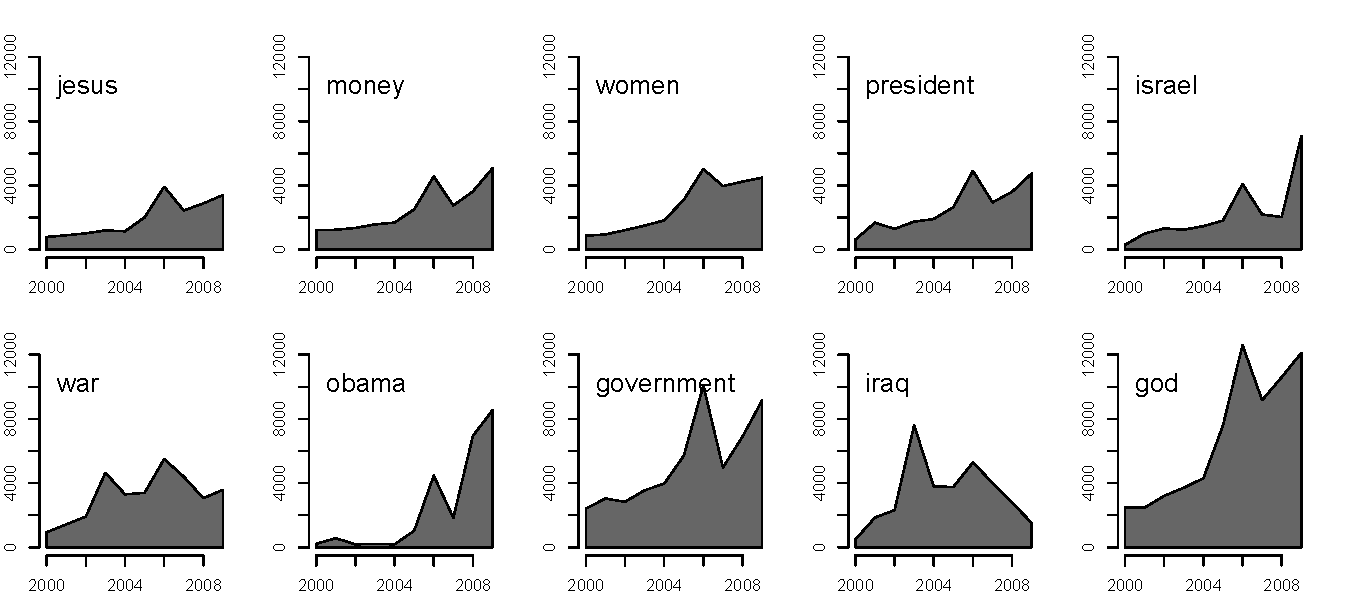
\includegraphics[width=18cm]{images/2by5_bigger3_small.pdf}
	\caption{Number of claims containing a particular noun made during January of any particular year}
	\label{multiplot_nouns}
	\end{center}
\end{figure*}

\subsection{Context}

We save the surrounding text, page title, and URL for each of the disputed claims we see made on the web. At present we do not do anything with this data, but we anticipate that it could be useful for many purposes; for example it may be possible to resolve the meaning of ambiguous words or entities based on the words nearby like Wikify~\cite{Mihalcea2007} does. Since many web sites have content written by multiple writers with different degrees of credibility, it is also useful to be able to know which writer disputed a particular claim. Other useful contextual information includes what organization hosted the page, who they link to, what meme-like phrases they make near to the claim, and whether the page is written in an ``expert'' style.

\section{Using Disputed Claims}
\label{using}

A corpus of disputed claims could be useful for many purposes, including real-time dispute recognition, background dispute analysis agents, and other research tools. Real-time dispute recognition agents could be used, for instance, to alert users when a trusted source disagrees with others, or to provide the user with feedback on how contentious a topic is.

Dispute Finder~\cite{Ennals2010} is one such agent that we are developing to provide real-time dispute recognition to users by identifying disputed claims that users encounter in their lives. The current implementation of Dispute Finder is a web browser extension that highlights text on web pages that appears to make a known disputed claim. In future research, we plan to extend Dispute Finder to be able to detect disputed information in television, and in speech that a user hears during conversations. We envision a device that provides real-time feedback to users regarding claims made in a conversation or presentation. Such a device would augment individuals' intuitive recognition of that a disputed claim is being made.

Dispute analysis agents that run in the background represent another application we see for a corpus of disputed claims. Such agents could be trained with information regarding the books, journals, and news articles a user reads. It would then be able to track these subjects and alert the user when a previously-read source is now disputed. It could also track a set of topics and tell the user when something new is disputed about a topic. A background dispute analysis agent would thus serve as an automated research assistant.

A third category of applications could be broadly classified as research tools: agents which allow users to explore what is disputed about a particular topic, or to more broadly examine the social dynamics of disputes on the web. As an increasing proportion of human knowledge is brought to the web, these tools will be increasingly important in sociological and historical research.

\section{Analyzing the Data}
\label{analysis}

\begin{figure}[tb]
	\begin{center}
	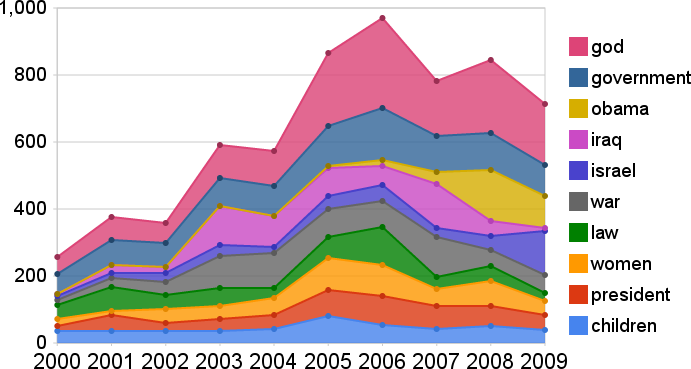
\includegraphics[width=8cm]{images/year_nouns.png}
	\caption{Frequency of different nouns on January 10th of various years}
	\label{year_nouns}
	\end{center}
\end{figure}


We downloaded all text strings that matched each of our 54 patterns for all dates from October 1st 2009 to January 19th 2010, and for January 10th of every year from 2000 to 2010. This gave us a total of 7 million text strings, of which 4.2 million were identified by our classifier as being unambiguous disputable claims. This does not mean that there are 4.2 million distinct beliefs that are disputed; many of the claims in our corpus are repeating claims made elsewhere in the corpus.

\subsection{Trends over time}
\label{timetrends}

Figure~\ref{multiplot_nouns} shows the frequency with which particular nouns were discussed in particular years. For example the claim ``Obama is a muslim'' contains the nouns ``Obama'' and ``Muslim''. We used the NLTK~\cite{Bird2009} part-of-speech tagger to identify the nouns found in each of our claims. We then analyzed the distribution of noun frequencies in claims made between January 1st and January 31st of every year from 2000 to 2010. Although the date we searched for was in January, the claims we found are often from other points in the year, due to the noisy nature of our date search mechanism (Figure~\ref{dateaccuracy}). We excluded uninteresting nouns such as ``someone'', ``anybody'' and ``something'', and plotted graphs for the ten most disputed nouns (Figure~\ref{multiplot_nouns}). All graphs are plotted on the same scale. The y axis is the number of claims that contained the noun, and the x axis is the year in which the claim was made. It is likely that a Named Entity Recognition algorithm~\cite{Nadeau2007} would produce better results, but even these nouns prove to be quite interesting.

We manually inspected our claims to determine what was going on that made particular nouns spike at particular times:

\begin{itemize}
 \item {\bf Obama:} Barack Obama is not a topic of dispute until 2004 when he spoke at the Democratic convention. His level of controversy then peaked in 2008, in the run up to the November 2008 US presidential elections. We believe that most of the mentions of Obama before 2004 are due to date classification errors.
 \item {\bf God:} God is always a controversial topic. We theorize that the spike in 2006 may relate to the 2006 publication of the Richard Dawkins book ``the God Delusion''\cite{Dawkins2006}.
 \item {\bf Iraq:} Spikes seem to correspond to the initial invasion in 2003 and the surge in 2007.
 \item {\bf Israel:} Spikes seem to correspond to the 2009 Gaza conflict and the 2006 Lebanon conflict.
\end{itemize}

These graphs are similar to those produced by MemeTracker~\cite{Backstrom2009}, which graphed when particular memes were discussed on the web. MemeTracker tracked highly repeated phrases, rather than nouns used in disputed claims. Kittur et al~\cite{Kittur2009} graphed the categories on Wikipedia that contained the most conflict.


\begin{figure}[tbh]
 \begin{center}
  \begin{tabular}{|lll|}
    \hline
    {\bf Noun} & {\bf Word Cluster} & {\bf Freq} \\
    \hline
   {\bf children} & tiger woods abused & 218\\
                  & instead encourage daily & 178\\
    \hline
   {\bf god} & daily encourage parents & 150 \\
   \hline
   {\bf government} & health care & 1267 \\
                    & united states & 427 \\
		    & relation environmental matters & 155 \\
   \hline
   {\bf iraq} & weapons mass destruction & 373 \\
              & united states & 247 \\
	      & saddam hussein & 192 \\
	      & al qaeda & 149 \\
   \hline
   {\bf israel} & middle east & 251 \\
		& allowed upon population & 128 \\
                & united states & 107 \\
		& off map & 106 \\
   \hline
   {\bf law}    & lawbreaker rather broken & 133 \\
		& united states & 116\\
   \hline
    {\bf obama} & working best interests & 568\\
                & health care & 481\\
	        & united states & 327 \\
		& nobel prize & 270 \\
		& legitimately president & 207 \\
		& fort hood shooter hasan nidal advised & 190 \\
		& birth certificate & 180\\
   \hline
   {\bf president} & united states & 439 \\
                   & health care & 203 \\
		   & george w & 164 \\
		   & aircraft system jolting bombing & 159 \\
		   & peace prize & 125 \\
		   & white house & 125 \\
   \hline
      {\bf war} & united states & 340 \\
   \hline

   {\bf women} & stay home & 183 \\
               & save vaccine & 85 \\
   \hline
  \end{tabular}
 \end{center}
 \caption{Largest word clusters found for nouns}
  \label{cluster-figure}

\end{figure}



\subsection{What is Disputed about a Noun?}
\label{clusters}

Once we know what nouns are disputed, it is interesting to know what it is about a noun that is disputed. For example, what is it that people are disputing about ``Obama'' or ``Iraq''? To address this question, we took the set of claims that contained each popular noun (e.g. ``Obama'') and looked for sets of words that occurred together much more frequently than would be expected if claims were formed randomly. For example in our claims about ``Obama'', we found the word cluster ``health care'' because most claims about Obama that contain the word ``health'' also contain the word ``care'' and vice-versa. We used an agglomerative clustering algorithm to group together words that co-occur in the same claims.

Figure~\ref{cluster-figure} shows the most frequently occurring word clusters that we found for each noun. For each cluster, the count is the number of claims about that noun that contain all of the words in the cluster. Most of these will make sense to people who have been following news in the United States. For example, we see that disputed claims about Obama often talk about his Nobel Prize or his birth certificate, and we see discussion about President Ahmadinejad's alleged statement that Israel should be wiped off the map (which the authors had not previously realized was a disputed). Some of the word clusters are not particularly interesting; for example many claims talk about the United States, even when that is not an important part of what is disputed. 

In the future, we plan to use ideas from textual entailment~\cite{Giampiccolo2007} to cluster claims together directly, and then automatically train a classifier that we can use to identify text that is making a disputed claim. This will allow us to better attack some of the problems we outlined in Section~\ref{using}.

\section{Conclusions}

Our research has shown that the web can be used as a corpus to determine what claims people identify as being disputed. Although it is likely that any specific claim found on the web is not authoritative, the web as a whole aggregates the collection of views that can be be found online. Furthermore, because individuals express opinions freely online, a snapshot of the disputed claims online can provide valuable insights into the cultural zeitgeist of the time.

Creating a comprehensive corpus of disputed claims presents many challenges: how to create patterns, how to search for patterns, how to avoid malformed sentences, how to resolve or filter out ambiguous claims, how to determine if two claims are paraphrases, and how to learn interesting things from the data set. For each of these tasks, we have implemented enough to get useful results, but there is much scope to do things better.

There are many possible applications for a corpus of disputed claims. These include real-time dispute recognition, autonomous research agents that operate in the background, and sociocultural research.

Our data set currently includes approximately 4.2 million records. In the future we intend to expand this by several orders of magnitude.


% mendelybib is the bibliograph from our shared mendely space and is auto-generated
% localbib is used for manually adding anything we don't want to add to mendeley, particularly for
% people who are not mendeley users
\bibliography{mendeleybib,localbib}

\end{document}


